\documentclass[a4paper,11pt]{article}
\usepackage{amsmath,amssymb,amsthm, tikz,titlesec,hyperref,esint,braket, graphicx}

\usepackage[a4paper,margin=2cm]{geometry}
\linespread{1.3}
\newtheorem{claim}{Claim}[section]

\newcommand\name{Park Chanwoo}   % Name of the student
\newcommand\university{KAIST} % Name of the university
\newcommand\department{Physics} % Name of the department
\newcommand\studentid{20230297} % Student ID
\newcommand\s{\,\;}


\newenvironment{solution}[1]
  {\renewcommand\qedsymbol{$\square$}\begin{proof}[\textbf{Solution#1}]}
  {\end{proof}}
\newenvironment{note}
  {\renewcommand\qedsymbol{$\blacksquare$}\begin{proof}[\textnormal{\textbf{note}}]}
  {\end{proof}}

\title{KAIST\\2025 PH361 Solid State Physics I\\
Homework 1\bigskip}
\author{\textbf{\Large \name} \\
% University: \university\\
Department: \department\\
Student ID: \studentid}
\date{\today}

\begin{document}
\thispagestyle{empty}
\maketitle
\tableofcontents
\titleformat{\section}[frame]{\pagebreak}{\filright
\footnotesize  \enspace \textsf{KAIST --- PH361 Solid State Physics I 2025 Spring}\enspace}{6pt}{\Large\bfseries\filcenter}

\newcommand{\der}[2][]{\frac{d #1}{d #2}}
\newcommand{\pder}[2][]{\frac{\partial #1}{\partial #2}}
\newcommand{\grad}{\operatorname{grad}}
\newcommand{\diver}{\operatorname{div}}
\newcommand{\curl}{\operatorname{curl}}
\newcommand{\boltz}{k_{\mathrm{B}}}
\newcommand{\tr}{\operatorname{tr}}
\newcommand{\Li}{\operatorname{Li}}

\section{2.7 Diatomic Einstein Solid}

\begin{note}

Let $\mathbf q$ and $\mathbf p \in \mathbb R$ be conjugated canonical coordinate and momentum in $2n$-dimensional phase space. For an arbitrary invertible linear transformation $A:\mathbb R^n \rightarrow \mathbb R^n$, $\mathbf Q = A\mathbf q; \mathbf P = (A^{-1})^\top\mathbf p$ is a canonical transformation. i.e., $AQ$
    
\end{note}

\begin{proof}
    The partial derivatives are:
    \begin{align}
        &\frac{\partial Q_i}{\partial q_j} = A_{ij},
        &\frac{\partial Q_i}{\partial p_j} = 0 \\
        &\frac{\partial P_i}{\partial q_j} = 0,
        &\frac{\partial P_i}{\partial p_j} = (A^{-1})_{ji}
    \end{align}
    so the Poisson braket is
    \begin{gather}
        \{Q_i, Q_j\} = \sum_{k=1}^n\left(\frac{\partial Q_i}{\partial q_k}\frac{\partial Q_j}{\partial p_k}-\frac{\partial Q_i}{\partial p_k}\frac{\partial Q_j}{\partial q_k}\right) = \sum_{k=1}^n\left(A_{ik}0-0A_{jk}\right) = 0\\
        \{P_i, P_j\} = \sum_{k=1}^n\left(\frac{\partial P_i}{\partial q_k}\frac{\partial P_j}{\partial p_k}-\frac{\partial P_i}{\partial p_k}\frac{\partial P_j}{\partial q_k}\right) = \sum_{k=1}^n\left(0(A^{-1})_{kj}-(A^{-1})_{ki}0\right) = 0\\
        \{Q_i, P_j\} = \sum_{k=1}^n\left(\frac{\partial Q_i}{\partial q_k}\frac{\partial P_j}{\partial p_k}-\frac{\partial Q_i}{\partial p_k}\frac{\partial P_j}{\partial q_k}\right)
        = \sum_{k=1}^n\left(A_{ik}(A^{-1})_{ki}-00\right) = (AA^{-1})_{ij}=  (I)_{ij}=\delta_{ij}
    \end{gather}

    Therefore, it is a canonical transformation.
\end{proof}

The Hamiltonian of the system is

\begin{align}
    H &= \frac{\|\mathbf{p}_1\|^2}{2m_1}
    + \frac{\|\mathbf{p}_2\|^2}{2m_2}
    + \frac{k}{2}\|\mathbf{x}_1\|^2
    + \frac{k}{2}\|\mathbf{x}_2\|^2
    + \frac{K}{2}\left\|\mathbf{x}_1 - \mathbf{x}_2\right\|^2 \\
    &= \frac{1}{2}\begin{pmatrix}\mathbf p_1^\top & \mathbf p_2^\top\end{pmatrix}
    \begin{pmatrix}1/{m_1}& 0 \\ 0 & 1/{m_2}\end{pmatrix}
    \begin{pmatrix}\mathbf p_1 \\ \mathbf p_2\end{pmatrix}
    + \frac{1}{2}\begin{pmatrix}\mathbf x_1^\top & \mathbf x_2^\top\end{pmatrix}
    \begin{pmatrix}k + K& -K \\ -K & k + K\end{pmatrix}
    \begin{pmatrix}\mathbf x_1 \\ \mathbf x_2\end{pmatrix}
\end{align}

Consider the canonical transformation.

\begin{equation}
    \begin{cases}
        \begin{pmatrix}\mathbf P_1 \\ \mathbf P_2\end{pmatrix}
        = 
        \begin{pmatrix} 1/\sqrt{m_1} & 0 \\ 0 & 1/\sqrt{m_2} \end{pmatrix}
        \begin{pmatrix}\cos\theta & -\sin\theta \\ \sin\theta & \cos\theta\end{pmatrix}
        \begin{pmatrix}\mathbf p_1 \\ \mathbf p_2\end{pmatrix}\\
        \begin{pmatrix}\mathbf Q_1 \\ \mathbf Q_2\end{pmatrix}
        = 
        \begin{pmatrix} \sqrt{m_1} & 0 \\ 0 & \sqrt{m_2}\end{pmatrix}
        \begin{pmatrix}\cos\theta & -\sin\theta \\ \sin\theta & \cos\theta\end{pmatrix}
        \begin{pmatrix}\mathbf x_1 \\ \mathbf x_2\end{pmatrix}
    \end{cases}
\end{equation}

Where
\begin{equation}
    \theta = \frac{1}{2}\arctan\left(\frac{2K\sqrt{m_1m_2}}{(m_1-m_2)(k + K)}\right)
\end{equation}

Then the Hamiltonian becomes the Hamiltonian of two decoupled 3D harmonic oscillators.

\begin{equation}
    H = \frac{1}{2}\mathbf \|\mathbf P_1\|^2 + \frac{1}{2}\mathbf \|\mathbf P_2\|^2+\frac{1}{2}\omega_+^2\|\mathbf Q_1\|^2+\frac{1}{2}\omega_-^2\|\mathbf Q_2\|^2
\end{equation}

Where
\begin{equation}
    \omega^2_{\pm} = \frac{k + K}{2}\left(\frac{1}{m_1} + \frac{1}{m_2}\right) \pm \sqrt{\left(\frac{k+K}{2}\left(\frac{1}{m_1} - \frac{1}{m_2}\right)\right)^2 + \frac{K^2}{m_1m_2}}
\end{equation}

and $\mathbf Q_1=(Q_1^x, Q_1^y, Q_1^z), \mathbf Q_2=(Q_2^x, Q_2^y, Q_2^z)$ and $\mathbf P_1=(P_1^x, P_1^y, P_1^z), \mathbf P_2=(P_2^x, P_2^y, P_2^z)$ are conjugated canonical coordinates and momentums.

(a) The classical partition function is Gaussian integral
\begin{align}
    Z &= \frac{1}{h^6}\int d^3\mathbf P_1 d^3\mathbf P_2 d^3\mathbf Q_1 d^3\mathbf Q_2
    e^{-\beta H(\mathbf P_1, \mathbf P_2, \mathbf Q_1, \mathbf Q_2)}\\
    &= \frac{1}{h^6}\int d^3\mathbf P_1 e^{-\frac{1}{2}\beta \mathbf P_1^2}\int d^3\mathbf P_2 e^{-\frac{1}{2}\beta \mathbf P_2^2}\int d^3\mathbf Q_1 e^{-\frac{1}{2}\beta \mathbf \omega^2_+Q_1^2}\int d^3\mathbf Q_2 e^{-\frac{1}{2}\beta \mathbf \omega^2_-Q_2^2}\\
    &=\frac{1}{h^6}\left(\sqrt{\frac{2\pi}{\beta}}\right)^6\left(\sqrt{\frac{2\pi}{\beta\omega_+^2}}\right)^3\left(\sqrt{\frac{2\pi}{\beta\omega_-^2}}\right)^3\\
    &=\frac{1}{(\hbar\omega_+)^3(\hbar\omega-)^3\beta^6}
\end{align}

The heat capacity is

\begin{equation}
    C = \frac{1}{\boltz T^2}\frac{\partial^2\log Z}{\partial \beta^2} = \frac{6}{\boltz T^2\beta^2}=6\boltz
\end{equation}

(b) Quantum mechanically, by introducing creation/annihilation operators and number operators, the Hamiltonian becomes

\begin{equation}
    H = \hbar\omega_+\left(n^x_1+n^y_1+n^z_1+\frac{3}{2}\right) + \hbar\omega_-\left(n^z_2+n^y_2+n^z_2+\frac{3}{2}\right)
\end{equation}
Where
\begin{gather}
    {a_1^{x}} = \sqrt{\frac{\omega_+}{2\hbar}}\left({Q_1^{x}}+\frac{i}{\omega_+}{P_1^{x}}\right),\quad 
    {a_1^{x}}^\dagger = \sqrt{\frac{\omega_+}{2\hbar}}\left({Q_1^{x}}-\frac{i}{\omega_+}{P_1^{x}}\right),\\
    {a_2^{x}} = \sqrt{\frac{\omega_-}{2\hbar}}\left({Q_2^{x}}+\frac{i}{\omega_-}{P_2^{x}}\right),\quad 
    {a_2^{x}}^\dagger = \sqrt{\frac{\omega_-}{2\hbar}}\left({Q_2^{x}}-\frac{i}{\omega_-}{P_2^{x}}\right),\\
    {n_1^{x}}={a_1^{x}}^\dagger {a_1^{x}},\quad {n_2^{x}}={a_2^{x}}^\dagger {a_2^{x}}
\end{gather}
Same for $y$ and $z$.

Since $[P_i^\alpha,P_j^{\beta}] = 0$, $[Q_i^\alpha,Q_j^{\beta}] = 0$, $[Q_i^\alpha,P_j^{\beta}] = i\hbar\delta_{(i, \alpha), (j, \beta)}$, the commutators of creation/annihilation operators are $[a_i^\alpha,a_j^{\beta}] = 0$, $[{a_i^\alpha}^\dagger,{a_j^{\beta}}^\dagger] = 0$, $[a_i^\alpha,{a_j^{\beta}}^\dagger] = \delta_{(i, \alpha), (j, \beta)}$, and the number operators are commute $[n_i^\alpha, n_j^\beta] = 0$.

Then the system is 6 decoupled 1D harmonic oscillators and the partition function is the product of the partition functions of 6 harmonic oscillators.
\begin{align}
    Z
    &= \left(\frac{1}{2\sinh\left(\beta\hbar\omega_+/2\right)}\right)^3\left(\frac{1}{2\sinh\left(\beta\hbar\omega_-/2\right)}\right)^3
\end{align}

The heat capacity is

\begin{align}
    C 
    &= \frac{1}{\boltz T^2}\frac{\partial^2\log Z}{\partial \beta^2} \\
    &= -\frac{3}{\boltz T^2}\frac{\partial^2}{\partial \beta^2}\log \sinh\left(\beta\hbar\omega_+/2\right)-\frac{3}{\boltz T^2}\frac{\partial^2}{\partial \beta^2}\log \sinh\left(\beta\hbar\omega_-/2\right)\\
    &=\frac{3\boltz\left(\beta\hbar\omega_+/2\right)^2}{\sinh^2\left(\beta\hbar\omega_+/2\right)} + \frac{3\boltz\left(\beta\hbar\omega_-/2\right)^2}{\sinh^2\left(\beta\hbar\omega_-/2\right)}\\
    &=\frac{3\boltz\left(\frac{\hbar\omega_+}{2\boltz T}\right)^2}{\sinh^2\left(\frac{\hbar\omega_+}{2\boltz T}\right)} + \frac{3\boltz\left(\frac{\hbar\omega_-}{2\boltz T}\right)^2}{\sinh^2\left(\frac{\hbar\omega_-}{2\boltz T}\right)}
\end{align}

\begin{figure}[!h]
    \centering
    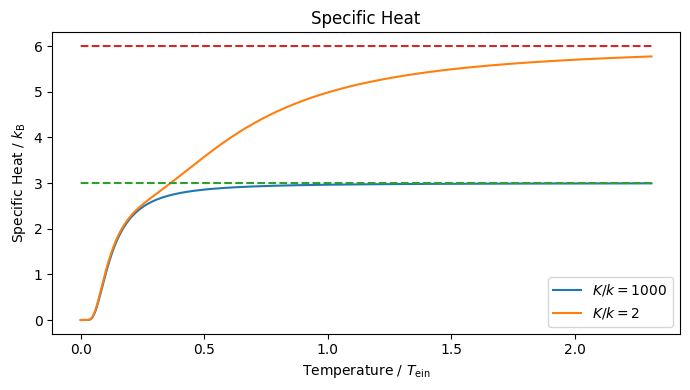
\includegraphics[width=0.5\linewidth]{image.png}
    \caption{Specific heat respect to the temperature.}
    \label{fig:specific-heat}
\end{figure}

If $k \ll K$, the molecule is tightly bonded so that it can be treated as a single molecule without any vibration mode at a low enough temperature. Figure.~\ref{fig:specific-heat} shows, that $K/k$ is large enough and the temperature is low enough, it shows $C=3\boltz$ which is the specific heat of a monatomic molecule.


(c) for the homogeneous diatomic molecule case, let $m_1 = m_2 = m$. Then,
\begin{align}
    H &= \frac{\|\mathbf{p}_1\|^2}{2m_1}
    + \frac{\|\mathbf{p}_2\|^2}{2m_2}
    + \frac{k}{2}\|\mathbf{x}_1\|^2
    + \frac{k}{2}\|\mathbf{x}_2\|^2
    + \frac{K}{2}\left\|\mathbf{x}_1 - \mathbf{x}_2\right\|^2 \\
    &= \frac{1}{2m}\begin{pmatrix}\mathbf p_1^\top & \mathbf p_2^\top\end{pmatrix}
    \begin{pmatrix}\mathbf p_1 \\ \mathbf p_2\end{pmatrix}
    + \frac{1}{2}\begin{pmatrix}\mathbf x_1^\top & \mathbf x_2^\top\end{pmatrix}
    \begin{pmatrix}k + K& -K \\ -K & k + K\end{pmatrix}
    \begin{pmatrix}\mathbf x_1 \\ \mathbf x_2\end{pmatrix}
\end{align}

In this case, consider only the rotation without scaling. Then transformation is
\begin{equation}
    \begin{cases}
        \begin{pmatrix}\mathbf P_1 \\ \mathbf P_2\end{pmatrix}
        = \frac{1}{\sqrt{2}}\begin{pmatrix}1 & 1 \\ 1 & -1 \end{pmatrix}
        \begin{pmatrix}\mathbf p_1 \\ \mathbf p_2\end{pmatrix}\\
        \begin{pmatrix}\mathbf Q_1 \\ \mathbf Q_2\end{pmatrix}
        = \frac{1}{\sqrt{2}}\begin{pmatrix}1 & 1 \\ 1 & -1 \end{pmatrix}
        \begin{pmatrix}\mathbf x_1 \\ \mathbf x_2\end{pmatrix}
    \end{cases}
\end{equation}

\begin{align}
    H 
    &= \frac{1}{2m}\mathbf \|\mathbf P_1\|^2 + \frac{1}{2m}\mathbf \|\mathbf P_2\|^2+\frac{1}{2}k\|\mathbf Q_1\|^2+\frac{1}{2}(k + 2K)\|\mathbf Q_2\|^2 \\
    &= \frac{1}{2m}\mathbf \|\mathbf P_1\|^2 + \frac{1}{2m}\mathbf \|\mathbf P_2\|^2+\frac{1}{2}m\omega_+^2\|\mathbf Q_1\|^2+\frac{1}{2}m\omega_-^2\|\mathbf Q_2\|^2
\end{align}
Where
\begin{equation}
    \omega_+=\omega=\sqrt{\frac{k}{m}},\quad \omega_-=\sqrt{\frac{k + 2K}{m}}
\end{equation}

Even in quantum mechanics, the Hamiltonian and position and momentum operators can be transformed similarly. The ladder operators can be defined by:
\begin{gather}
    a_+^x 
    = \sqrt{\frac{m\omega_+}{2\hbar}}\left(Q_1^x+\frac{i}{m\omega_+}P_1^x\right) \\
    a_-^x 
    = \sqrt{\frac{m\omega_-}{2\hbar}}\left(Q_2^x-\frac{i}{m\omega_-}P_2^x\right)
\end{gather}
same for $y$ and $z$

Let $\Pi$ be the permutation operator:
\begin{equation}
    \bra{\mathbf x_1, \mathbf x_2}\Pi\ket{\psi} = \braket{\mathbf x_2, \mathbf x_1|\psi}
\end{equation}

Then the commutator and anti-commutators are relations holds:
\begin{align}
    \bra{\mathbf x_1', \mathbf x_2'}[\Pi, Q_1^x]\ket{\psi}
    &= \bra{\mathbf x_1', \mathbf x_2'}\Pi Q_1^x - Q_1^x\Pi\ket{\psi} \\
    &= \bra{\mathbf x_1', \mathbf x_2'}\Pi \frac{x_1+x_2}{\sqrt{2}}\ket{\psi} - \bra{\mathbf x_1', \mathbf x_2'}\frac{x_1+x_2}{\sqrt{2}}\Pi\ket{\psi}\\
    &= \bra{\mathbf x_2', \mathbf x_1'}\frac{x_1+x_2}{\sqrt{2}}\ket{\psi} - \frac{x_1'+x_2'}{\sqrt{2}}\bra{\mathbf x_1', \mathbf x_2'}\Pi\ket{\psi}\\
    &= \frac{x_2'+x_1'}{\sqrt{2}}\braket{\mathbf x_2', \mathbf x_1'|\psi} - \frac{x_1+x_2}{\sqrt{2}}\bra{\mathbf x_2', \mathbf x_1'}\Pi\ket{\psi}\\
    &= 0
\end{align}
\begin{align}
    \bra{\mathbf x_1', \mathbf x_2'}\{\Pi, Q_2^x\}\ket{\psi}
    &= \bra{\mathbf x_1', \mathbf x_2'}\Pi Q_2^x + Q_2^x\Pi\ket{\psi} \\
    &= \bra{\mathbf x_1', \mathbf x_2'}\Pi \frac{x_1-x_2}{\sqrt{2}}\ket{\psi} + \bra{\mathbf x_1', \mathbf x_2'}\frac{x_1-x_2}{\sqrt{2}}\Pi\ket{\psi}\\
    &= \bra{\mathbf x_2', \mathbf x_1'}\frac{x_1-x_2}{\sqrt{2}}\ket{\psi} + \frac{x_1'-x_2'}{\sqrt{2}}\bra{\mathbf x_1', \mathbf x_2'}\Pi\ket{\psi}\\
    &= \frac{x_2'-x_1'}{\sqrt{2}}\braket{\mathbf x_2', \mathbf x_1'|\psi} + \frac{x_1-x_2}{\sqrt{2}}\bra{\mathbf x_2', \mathbf x_1'}\Pi\ket{\psi}\\
    &= 0
\end{align}

Similar things are hold for momentum operators.

\begin{align}
    \bra{\mathbf x_1', \mathbf x_2'}[\Pi, P_1^x]\ket{\psi}
    &= \bra{\mathbf x_1', \mathbf x_2'}\Pi P_1^x - P_1^x\Pi\ket{\psi} \\
    &= \bra{\mathbf x_1', \mathbf x_2'}\Pi \frac{p_1+p_2}{\sqrt{2}}\ket{\psi} - \bra{\mathbf x_1', \mathbf x_2'}\frac{p_1+p_2}{\sqrt{2}}\Pi\ket{\psi}\\
    &= \bra{\mathbf x_2', \mathbf x_1'}\frac{p_1+p_2}{\sqrt{2}}\ket{\psi} + \frac{i\hbar}{\sqrt{2}}\left(\frac{\partial}{\partial x_1} + \frac{\partial}{\partial x_2}\right)\bra{\mathbf x_1', \mathbf x_2'}\Pi\ket{\psi}\\
    &= - \frac{i\hbar}{\sqrt{2}}\left(\frac{\partial}{\partial x_2} + \frac{\partial}{\partial x_1}\right)\braket{\mathbf x_2', \mathbf x_1'|\psi} + \frac{i\hbar}{\sqrt{2}}\left(\frac{\partial}{\partial x_1} + \frac{\partial}{\partial x_2}\right)\bra{\mathbf x_2', \mathbf x_1'}\Pi\ket{\psi}\\
    &= 0
\end{align}
\begin{align}
    \bra{\mathbf x_1', \mathbf x_2'}\{\Pi, P_2^x\}\ket{\psi}
    &= \bra{\mathbf x_1', \mathbf x_2'}\Pi P_2^x + P_2^x\Pi\ket{\psi} \\
    &= \bra{\mathbf x_1', \mathbf x_2'}\Pi \frac{p_1-p_2}{\sqrt{2}}\ket{\psi} + \bra{\mathbf x_1', \mathbf x_2'}\frac{p_1-p_2}{\sqrt{2}}\Pi\ket{\psi}\\
    &= \bra{\mathbf x_2', \mathbf x_1'}\frac{p_1-p_2}{\sqrt{2}}\ket{\psi} - \frac{i\hbar}{\sqrt{2}}\left(\frac{\partial}{\partial x_1} - \frac{\partial}{\partial x_2}\right)\bra{\mathbf x_1', \mathbf x_2'}\Pi\ket{\psi}\\
    &= - \frac{i\hbar}{\sqrt{2}}\left(\frac{\partial}{\partial x_2} - \frac{\partial}{\partial x_1}\right)\bra{\mathbf x_2', \mathbf x_1'}\braket{\mathbf x_2', \mathbf x_1'|\psi} - \frac{i\hbar}{\sqrt{2}}\left(\frac{\partial}{\partial x_1} - \frac{\partial}{\partial x_2}\right)\bra{\mathbf x_2', \mathbf x_1'}\Pi\ket{\psi}\\
    &= 0
\end{align}

Therfore, $[\Pi, Q_1^x]=0$, $\{\Pi, Q_2^x\}=0$, $[\Pi, P_1^x]=0$ and $\{\Pi, P_2^x\}=0$ are holds. 

This relation can be extended to ladder operators.
\begin{gather}
    [\Pi, (a_+^x)^\dagger] = \left[\Pi, \sqrt\frac{m\omega}{2\hbar}\left(Q_1^x-\frac{i}{m\omega}P_1^x\right)\right]= \sqrt\frac{m\omega}{2\hbar}\left([\Pi, Q_1^x]-\frac{i}{m\omega}[\Pi, P_1^x]\right)=0\\
    \{\Pi, (a_-^x)^\dagger\} = \left\{\Pi, \sqrt\frac{m\omega}{2\hbar}\left(Q_2^x-\frac{i}{m\omega}P_2^x\right)\right\}= \sqrt\frac{m\omega}{2\hbar}\left(\{\Pi, Q_2^x\}-\frac{i}{m\omega}\{\Pi, P_2^x\}\right)=0
\end{gather}
The same things are held for $y$ and $z$.

Also, the ground state is symmetrized.
\begin{equation}
    \Pi\ket{\text{GS}} = \Pi\ket{0}\otimes\ket{0}=\ket{0}\otimes\ket{0}
\end{equation}

Hence,
\begin{align}
    \Pi\ket{n_+^x,n_+^y,n_+^z, n_-^x,n_-^y,n_-^z}
    &=\Pi\frac{{(a_+^x)^\dagger}^{n_+^x}}{\sqrt{n_+^x!}}\frac{{(a_+^x)^\dagger}^{n_+^x}}{\sqrt{n_+^y!}}\frac{{(a_+^y)^\dagger}^{n_+^z}}{\sqrt{n_+^z!}}\frac{{(a_-^x)^\dagger}^{n_-^x}}{\sqrt{n_-^x!}}\frac{{(a_-^x)^\dagger}^{n_-^x}}{\sqrt{n_-^y!}}\frac{{(a_-^y)^\dagger}^{n_-^z}}{\sqrt{n_-^z!}}\ket{\text{GS}} \\
    &=(-1)^{n_-^x+n_-^y+n_-^z}\frac{{(a_+^x)^\dagger}^{n_+^x}}{\sqrt{n_+^x!}}\frac{{(a_+^x)^\dagger}^{n_+^x}}{\sqrt{n_+^y!}}\frac{{(a_+^y)^\dagger}^{n_+^z}}{\sqrt{n_+^z!}}\frac{{(a_-^x)^\dagger}^{n_-^x}}{\sqrt{n_-^x!}}\frac{{(a_-^x)^\dagger}^{n_-^x}}{\sqrt{n_-^y!}}\frac{{(a_-^y)^\dagger}^{n_-^z}}{\sqrt{n_-^z!}}\Pi\ket{\text{GS}}\\
    &=(-1)^{n_-^x+n_-^y+n_-^z}\frac{{(a_+^x)^\dagger}^{n_+^x}}{\sqrt{n_+^x!}}\frac{{(a_+^x)^\dagger}^{n_+^x}}{\sqrt{n_+^y!}}\frac{{(a_+^y)^\dagger}^{n_+^z}}{\sqrt{n_+^z!}}\frac{{(a_-^x)^\dagger}^{n_-^x}}{\sqrt{n_-^x!}}\frac{{(a_-^x)^\dagger}^{n_-^x}}{\sqrt{n_-^y!}}\frac{{(a_-^y)^\dagger}^{n_-^z}}{\sqrt{n_-^z!}}\ket{\text{GS}}\\
    &=(-1)^{n_-^x+n_-^y+n_-^z}\ket{n_+^x,n_+^y,n_+^z, n_-^x,n_-^y,n_-^z}    
\end{align}



The energy eigenstates are already the $\pm 1$ eigenstates of $\Pi$, i.e. they are symmetrized or anti-symmetrized. if $n_-^x+n_-^y+n_-^z$ is even, the state is bosonic, $n_-^x+n_-^y+n_-^z$ is odd, the state is fermionic, 

i) bosonic case
\begin{align}
    Z &= \tr e^{-\beta H} \\
    &= \sum_{\text{$n_-^x+n_-^y+n_-^z$ is even}} e^{-\beta E(n_+^x,n_+^y,n_+^z, n_-^x,n_-^y,n_-^z)} \\
    &= \sum_{\text{$n_-^x+n_-^y+n_-^z$ is even}} e^{-\beta \hbar\omega_+(n_+^x + n_+^y + n_+^z + 3/2)}e^{\hbar\omega_-(n_-^x + n_-^y + n_-^z + 3/2)} \\
    &= \sum e^{-\beta \hbar\omega_+(n_+^x + n_+^y + n_+^z + 3/2)} \sum_{\text{$n_-^x+n_-^y+n_-^z$ is even}} e^{\hbar\omega_-(n_-^x + n_-^y + n_-^z + 3/2)}
\end{align}

Use the known value for the 3D harmonic oscillator.

\begin{equation}
    Z = \left(\frac{1}{2\sinh(\beta\hbar\omega_+/2)}\right)^3\sum_{\text{$n_-^x+n_-^y+n_-^z$ is even}} e^{-\hbar\omega_-(n_-^x + n_-^y + n_-^z + 3/2)}
\end{equation}

Since $(1 + (-1)^{-(n_-^x + n_-^y + n_-^z)}) / 2$ is $1$ if and only if $n_-^x + n_-^y + n_-^z$ is even, modify the summation.

\begin{align}
    Z &= \left(\frac{1}{2\sinh(\beta\hbar\omega_+/2)}\right)^3\sum \frac{(1 + (-1)^{-(n_-^x + n_-^y + n_-^z)})}{2}e^{-\hbar\omega_-(n_-^x + n_-^y + n_-^z + 3/2)}\\
    &= \frac{1}{2}\left(\frac{1}{2\sinh(\beta\hbar\omega_+/2)}\right)^3\left[\sum e^{-\hbar\omega_-(n_-^x + n_-^y + n_-^z + 3/2)}+ \sum (-1)^{-(n_-^x + n_-^y + n_-^z)}e^{-\hbar\omega_-(n_-^x + n_-^y + n_-^z + 3/2)}\right]
\end{align}

For the left term, use the result of THE 3D harmonic oscillator; for the right term, use the geometric series formula.

\begin{align}
    Z&= \frac{1}{2}\left(\frac{1}{2\sinh(\beta\hbar\omega_+/2)}\right)^3\left[\left(\frac{1}{2\sinh(\beta\hbar\omega_-/2)}\right)^3 +\left(\frac{e^{-\beta\hbar\omega_-/2}}{1+e^{-\beta\hbar\omega_-/2}}\right)^3\right] \\
    &= \frac{1}{2}\left(\frac{1}{2\sinh(\beta\hbar\omega_+/2)}\right)^3\left[\left(\frac{1}{2\sinh(\beta\hbar\omega_-/2)}\right)^3 +\left(\frac{1}{2\cosh(\beta\hbar\omega_-/2)}\right)^3\right]
\end{align}

The heat capacity is
\begin{align}
    C 
    &= \frac{1}{\boltz T^2}\frac{\partial^2\log Z}{\partial \beta^2} \\
    &= \frac{3\boltz\left(\frac{\hbar \omega_+}{2\boltz T}\right)^2}{\sinh^2\left(\frac{\hbar\omega_+}{2\boltz T}\right)} + \frac{6 \beta^{2} \omega_{-}^{2} \hbar^{2} k_{B} \left(- 2 \sinh{\left(2 \beta \omega_{-} \hbar \right)} + 3 \cosh{\left(2 \beta \omega_{-} \hbar \right)} + 1\right)}{\left(\sinh{\left(\beta \omega_{-} \hbar \right)} - 2 \cosh{\left(\beta \omega_{-} \hbar \right)}\right)^{2} \left(\cosh{\left(2 \beta \omega_{-} \hbar \right)} - 1\right)}
\end{align}
    
ii) fermionic case

In a similar way, for this case, introduce $(1 - (-1)^{-(n_-^x + n_-^y + n_-^z)}) / 2$ which is 1 if and only if $n_-^x + n_-^y + n_-^z$ is odd. the only change is the sign.

\begin{equation}
    Z= \frac{1}{2}\left(\frac{1}{2\sinh(\beta\hbar\omega_+/2)}\right)^3\left[\left(\frac{1}{2\sinh(\beta\hbar\omega_-/2)}\right)^3 -\left(\frac{1}{2\cosh(\beta\hbar\omega_-/2)}\right)^3\right]
\end{equation}

The heat capacity is
\begin{align}
    C 
    &= \frac{1}{\boltz T^2}\frac{\partial^2\log Z}{\partial \beta^2} \\
    &= \frac{3\boltz\left(\frac{\hbar \omega_+}{2\boltz T}\right)^2}{\sinh^2\left(\frac{\hbar\omega_+}{2\boltz T}\right)} + \frac{6 \beta^{2} \omega_{-}^{2} \hbar^{2} k_{B} \left(2 \sinh{\left(2 \beta \omega_{-} \hbar \right)} + 3 \cosh{\left(2 \beta \omega_{-} \hbar \right)} + 1\right)}{\left(\sinh{\left(\beta \omega_{-} \hbar \right)} + 2 \cosh{\left(\beta \omega_{-} \hbar \right)}\right)^{2} \left(\cosh{\left(2 \beta \omega_{-} \hbar \right)} - 1\right)}
\end{align}








\section{3.1 Drude Theory of Transport in Metals}

From the assumptions of the Drude theory,
\begin{gather}
    \braket{\mathbf p(t+dt)} = \left(1 - \frac{dt}{\tau}\right)\left(\mathbf p(t) + \mathbf Fdt\right) + 0\frac{dt}{\tau}\\
    \frac{d\mathbf p}{dt}=\mathbf F-\frac{\mathbf p}{\tau}=-e\mathbf E-e\mathbf v\times\mathbf B-\frac{\mathbf p}{\tau}
\end{gather}

Assume the steady-state and no external magnetic field
\begin{gather}
    -e\mathbf E -\frac{\mathbf p}{\tau} = 0\\
    m\mathbf v = \mathbf p = -e\tau\mathbf E
\end{gather}

Introduce the number density $n$ and use the identity $\mathbf j = -en\mathbf v$
\begin{equation}
    \mathbf j = \frac{e^2\tau n}{m}\mathbf E
\end{equation}

(a) Hence the conductivity is 
\begin{equation}
    \sigma =\frac{e^2\tau n}{m}
\end{equation}

(b) In the presence of the magnetic field,

\begin{gather}
    -e\mathbf E+-e\mathbf v\times\mathbf B-\frac{\mathbf p}{\tau} = 0 \\
    \mathbf E = \frac{1}{en}\mathbf j\times\mathbf B+\frac{m\mathbf j}{e^2\tau n} \\
    \mathbf E_i = \frac{1}{en}(\mathbf j\times\mathbf B)_i+\frac{m}{e^2\tau n}\mathbf j_i= \frac{1}{en}\varepsilon_{ijk}\mathbf j_j\mathbf B_k+\frac{m}{e^2\tau n}\delta_{ij}\mathbf j_j
\end{gather}

Hence, 
\begin{equation}
    \underset{\sim}{\rho} = \begin{pmatrix}
        \frac{m}{e^2\tau n} & \frac{B_z}{en} & -\frac{B_y}{en}\\
        -\frac{B_z}{en} & \frac{m}{e^2\tau n} & \frac{B_x}{en} \\
        \frac{B_y}{en} & -\frac{B_x}{en} & \frac{m}{e^2\tau n} 
    \end{pmatrix}
\end{equation}
and the conductivity is $$\underset{\sim}{\sigma} = \underset{\sim}{\rho}^{-1}$$, 
\begin{gather}
    \frac{\tau e^{2} n}{m \left(\tau^{2} e^{2} \left(B_{x}^{2} + B_{y}^{2} + B_{z}^{2}\right) + m^{2}\right)} 
    \begin{pmatrix}B_{x}^{2} \tau^{2} e^{2} + m^{2} & \tau e \left(B_{x} B_{y} \tau e - B_{z} m\right) & \tau e \left(B_{x} B_{z} \tau e + B_{y} m\right)\\\tau e \left(B_{x} B_{y} \tau e + B_{z} m\right) & B_{y}^{2} \tau^{2} e^{2} + m^{2} & \tau e \left(- B_{x} m + B_{y} B_{z} \tau e\right)\\\tau e \left(B_{x} B_{z} \tau e - B_{y} m\right) & \tau e \left(B_{x} m + B_{y} B_{z} \tau e\right) & B_{z}^{2} \tau^{2} e^{2} + m^{2}\end{pmatrix}
\end{gather}

put $B_x=B_y=0$
\begin{gather}
    \frac{\tau e^{2} n}{m \left(\tau^{2} e^{2} B_{z}^{2} + m^{2}\right)} 
    \begin{pmatrix}
    m^{2} & -\tau e B_{z} m & 0\\
    \tau e B_{z} m & m^{2} & 0\\
    0 & 0 & B_{z}^{2} \tau^{2} e^{2} + m^{2}
    \end{pmatrix}
\end{gather}


(c)
The Hall coefficient $R_H$ is defined as
\begin{equation}
    R_H = \frac{\rho_{xy}}{|B|}
\end{equation}

For the Drude model,
\begin{equation}
    R_H = -\frac{1}{en}
\end{equation}

Sodium has $(6.022\times10^{23}\ \mathrm{mol}^{-1})(1\ \mathrm{g}\cdot\mathrm{cm}^{-3})(1\ \mathrm{cm}^3)/(23\  \mathrm{g}\cdot\mathrm{mol}^{-1}) = 2.618×10^{22}$ atoms. Hence the number density of the free electron of sodium is $n = 2.618×10^{28}\ \mathrm{m^{-3}}$

Since the cross-sectional area of the rod is $L^2$, where $L = 5 \times 10^{-3} m$, the current density is $j=I/L^2$. The hall voltage is $E_\text{cross}L=BR_Hj={IB/neL}=4.768 \times 10^{-8}\ \mathrm{V}$.

The hall voltage is very small. so we need a very accurate voltage meter. This can be replaced by using an alternating current circuit and an amplifier such as a lock-in amplifier.

(d)
\begin{itemize}
    \item At high frequency ($\sim 1/\tau$) it may be failed. 
    \item The model is classical. This model does not include Fermi-Dirac statistics. So, the model cannot expect the specific heat accurately.
\end{itemize}

(e) put the time-harmonic uniform fields $\mathbf Ee^{i\omega t}$, $\mathbf je^{i\omega t}$ to the equation
\begin{equation}
    \frac{d\mathbf p}{dt}=-\frac{m}{en}\frac{d\mathbf j e^{i\omega t}}{dt}=-e\mathbf Ee^{i\omega t} +\frac{1}{n}\mathbf j\times \mathbf Be^{i\omega t}
\end{equation}

the equation of motion is
\begin{gather}
    -i\frac{m\omega}{en}\mathbf je^{i\omega t}=-e{\mathbf E}e^{i\omega t} +\frac{B}{n}\mathbf j\times \hat{\mathbf z}e^{i\omega t} \\
    {\mathbf E}=i\frac{m\omega}{e^2n}\mathbf j +\frac{1}{en}\mathbf j\times {\mathbf B}
\end{gather}

The scattering rate is changed from the previous result $1/\tau\rightarrow i\omega$.

Hence,
\begin{equation}
    \underset{\sim}{\rho} = \begin{pmatrix}
        \frac{im\omega}{e^2 n} & \frac{B_z}{en} & -\frac{B_y}{en}\\
        -\frac{B_z}{en} & \frac{im\omega}{e^2 n} & \frac{B_x}{en} \\
        \frac{B_y}{en} & -\frac{B_x}{en} & \frac{im\omega}{e^2 n} 
    \end{pmatrix}
\end{equation}
and the conductivity is $$\underset{\sim}{\sigma} = \underset{\sim}{\rho}^{-1}$$, 
\begin{multline}
    \frac{i\omega e^{2} n}{m \left(e^{2} \left(B_{x}^{2} + B_{y}^{2} + B_{z}^{2}\right) - m^{2}\omega^2\right)} \times \\
    \begin{pmatrix}
    -B_{x}^{2} 
    e^{2}/\omega^2 + m^{2} 
    & -i e \left(-iB_{x} B_{y} e/\omega - B_{z} m\right)/\omega 
    & -i e \left(-iB_{x} B_{z} e/\omega + B_{y} m\right)/\omega\\
    -i e \left(-iB_{x} B_{y} e/\omega + B_{z} m\right)/\omega 
    & -B_{y}^{2} e^{2}/\omega^2 + m^{2} 
    & -i e \left(-iB_{y} B_{z} e/\omega - B_{x} m\right)/\omega\\
    -i e \left(-iB_{x} B_{z} e/\omega - B_{y} m\right)/\omega 
    & -i e \left(B_{x} m + -iB_{y} B_{z} e/\omega\right)/\omega 
    & -B_{z}^{2} e^{2}/\omega^2 + m^{2}
    \end{pmatrix}
\end{multline}

put $B_x=B_y=0$
\begin{gather}
    \frac{i\omega e^{2} n}{m \left(e^{2} B_{z}^{2} - m^{2}\omega^2\right)} 
    \begin{pmatrix}
    m^{2} & ie B_{z} m/\omega & 0\\
    -ie B_{z} m/\omega & m^{2} & 0\\
    0 & 0 & -B_{z}^{2} e^{2}/\omega^2 + m^{2}
    \end{pmatrix}
\end{gather}

When $\omega = eB/m$, the cyclotron frequency, it diverges. 

If the resistivities diverge, the electromagnetic waves will decay very quickly, so experimentally find this point, and use known $e$, $B$ to find the mass of the electron. 

\section{4.2 Velocities in the Free Electron Theory}

(a)
For the free particles in a box with periodic boundary condition, the energy spectrum is

\begin{equation}
    E = \frac{\hbar^2 \|\mathbf k\|^2}{2m}
\end{equation}

Where $\mathbf k = \mathbf n\pi/L$, $\mathbf n\in\mathbb Z^d$

From this relation, we can define Fermi-wavenumber:
\begin{equation}
    E_F = \frac{\hbar^2k_F^2}{2m}
\end{equation}

The relation between $k$ and $v$ is
\begin{equation}
    v=\frac{p}{m}=\frac{hk}{m}
\end{equation}

Fermi-velocity also defined by
\begin{equation}
    v_F = \frac{\hbar k_F}{m}
\end{equation}

Then the number of electrons occupied below the Fermi-energy can be expressed by
\begin{equation}
    N = \sum_{k\leq k_F, \sigma=\uparrow, \downarrow} 1
\end{equation}

Replace the summation to the integral on the thermodynamic limit: $\sum\rightarrow \frac{L}{2\pi}\int$

\begin{equation}
    N = 2\frac{V}{(2\pi)^d}\int_{k\leq k_f} d^dk
\end{equation}

Consider the three-dimensional case: $d=3$
\begin{equation}
    N = 2\frac{V}{(2\pi)^3}\int_{k\leq k_f} d^3k = 2\frac{V}{8\pi^3}\frac{4}{3}\pi k_F^3 = \frac{Vk_F^3}{3\pi^2}
\end{equation}

let $n = N/V$ be the number density:
\begin{equation}
    n = \frac{N}{V} = \frac{k_F^3}{3\pi^2} = \frac{m^3v_F^3}{3\hbar^3\pi^2}
\end{equation}

Hence, the fermi velocity is
\begin{equation}
    v_F = \frac{\hbar}{m}(3\pi^2 n)^{1/3}
\end{equation}

(b)
The electric current driven by electron is given by
\begin{equation}
    \mathbf j=\rho\mathbf v = -en\mathbf v
\end{equation}
and the Ohm's law is

\begin{equation}
    \mathbf j=\sigma\mathbf E
\end{equation}

Hence, 
\begin{equation}
    |\sigma\mathbf E|=|en\mathbf v|=|en|v_d
\end{equation}

Therefore, the mean drift speed is
\begin{equation}
    v_d=\left|\frac{\sigma E}{ne}\right|
\end{equation}

From the Drude theory,
\begin{equation}
    \sigma = \frac{e^2\tau n}{m}
\end{equation}

The relation between the scattering time and mean free path is
\begin{equation}
    \lambda=v\tau
\end{equation}

Take the velocity $v=v_F$. Then the equation becomes
\begin{equation}
    \sigma = ne^2\frac{\lambda}{mv_F}.
\end{equation}

(c.i) 
\begin{equation}
    v_d=\left|\frac{\sigma E}{ne}\right| = 4.358 \times 10^{-3}\ \mathrm{m} \cdot \mathrm{s}^{-1}
\end{equation}

\begin{equation}
    v_F = \frac{\hbar}{m}(3\pi^2 n)^{1/3} = 1.572 \times 10^{6}\ \mathrm{m} \cdot \mathrm{s}^{-1}
\end{equation}

The fermi velocity is much faster than the drift velocity.

(c.ii)
the fermi temperature of the copper is
\begin{equation}
    T_F=\frac{1}{\boltz}\frac{\hbar^2k_F^2}{2m}=\frac{1}{\boltz}\frac{\hbar^2(3\pi^2n)^{2/3}}{2m} \approx 81528\ \mathrm{K} \gg 300\ \mathrm{K}
\end{equation}
Hence, room temperature can be treated as zero temperature. So, it is reasonable to assume that $v=v_F$ in (b).
\begin{equation}
    \lambda = \sigma\frac{mv_F}{ne^2} = 3.896\times10^{-8}\ \mathrm{m}
\end{equation}



\section{4.8 Heat Capacity of a Free Electron Gas}

(a) for the noninteracting Fermi gas, the grand canonical partition function is

\begin{equation}
    Z = \prod_{i}\left(1 + e^{-\beta(\varepsilon_i -\mu)}\right)
\end{equation}

electron is spin-1/2, and the energy spectrum is
\begin{equation}
    \varepsilon(\mathbf k)=\frac{\hbar^2\|\mathbf k\|^2}{2m}, \quad \mathbf k=\frac{\mathbf n\pi}{L}, \mathbf n\in\mathbb Z^d
\end{equation}

Hence the partition function is
\begin{align}
    \Xi 
    &= \prod_{\mathbf k, \sigma}\left(1 + e^{-\beta(\varepsilon(\mathbf k) -\mu)}\right) \\
    &= \left(\prod_{\mathbf k}\left(1+ e^{-\beta\left(\frac{\hbar^2\|\mathbf{k}\|^2}{2m} -\mu\right)}\right)\right)^2
\end{align}
and
\begin{equation}
    \log \Xi 
     = 2\sum_{\mathbf k} \log\left(1+ e^{-\beta\left(\frac{\hbar^2\|\mathbf{k}\|^2}{2m} -\mu\right)}\right)
\end{equation}

% The grand potential is
% \begin{align}
%     \Phi 
%     &= -\frac{1}{\beta}\log \Xi \\
%     &= -\frac{1}{\beta}\left(2\sum_{n_x, n_y, n_z} \log\left(1+ e^{-\beta\left(\frac{\pi^2\hbar^2}{2mL^2}(n_x^2+n_y^2+n_z^2) -\mu\right)}\right)\right)
% \end{align}

The expected energy is
\begin{align}
    \braket{E}&=-\frac{\partial\log\Xi}{\partial \beta}+\frac{\mu}{\beta}\frac{\partial\log\Xi}{\partial \mu} \\
    &=2\sum_{\mathbf{k}}\frac{\varepsilon(\mathbf k)}{1 + e^{\beta(\varepsilon(\mathbf k) - \mu)}}
\end{align}

convert the summation to the integral 
\begin{align}
    \braket{E}
    &=2\left(\frac{L}{2\pi}\right)^2\int d^2\mathbf k \frac{\varepsilon(\mathbf k)}{1 + e^{\beta(\varepsilon(\mathbf k) - \mu)}} \\
    &=\frac{V}{2\pi^2}\int_0^\infty 2\pi k dk \frac{\varepsilon(\mathbf k)}{1 + e^{\beta(\varepsilon(\mathbf k) - \mu)}}\\
    &=\frac{Vm}{\pi\hbar^2}\int_0^\infty d\varepsilon \frac{\varepsilon}{1 + e^{\beta(\varepsilon - \mu)}}\\
    &=-\frac{Vm}{\pi\hbar^2}\frac{1}{\beta^2}\Li_2(-e^{\beta\mu})\\
    &=-\frac{Vm\boltz^2}{\pi\hbar^2}T^2\Li_2(-e^{\mu/\boltz T})
\end{align}
Where $\Li_2$ is the polylogarithm function of order 2, which is the analytic continuation of $f(z)=-\int_{0}^{z}\frac{\ln(1-u)}{u}du$.

The Fermi-Dirac integration
\begin{equation}
    F_j(x)=\frac{1}{\Gamma(j+1)}\int_0^\infty\frac{t^j}{e^{t-x} + 1}dt = -\Li_{j+1}(-e^x)
\end{equation}
is used.

The specific heat is
\begin{equation}
    C=\frac{\partial\braket{E}}{\partial T} = 2 T \Li_{2}\left(- e^{\frac{\mu}{T k_{B}}}\right) + \frac{\mu \log{\left(e^{\frac{\mu}{T k_{B}}} + 1 \right)}}{k_{B}}
\end{equation}

(b)
Convert it into 3-dimensional case.
\begin{align}
    \braket{E}
    &=2\left(\frac{L}{2\pi}\right)^3\int d^3\mathbf k \frac{\varepsilon(\mathbf k)}{1 + e^{\beta(\varepsilon(\mathbf k) - \mu)}} \\
    &=\frac{V}{4\pi^3}\int 4\pi k^2 d k \frac{\varepsilon(\mathbf k)}{1 + e^{\beta(\varepsilon(\mathbf k) - \mu)}} \\
    &= \frac{\sqrt{2}m^{3/2}V}{\pi^2\hbar^3}\int d\varepsilon \frac{\varepsilon^{3/2}}{1 + e^{\beta(\varepsilon - \mu)}} \\
    &= -\frac{\sqrt{2}m^{3/2}V}{\pi^2\hbar^3}\frac{3\sqrt{\pi}}{4\beta^{5/2}}\Li_{5/2}\left(-e^{\beta\mu}\right)\\
    &= -\frac{3\sqrt{2}m^{3/2}V\boltz^{5/2}}{4\pi^{3/2}\hbar^3}T^{5/2}\Li_{5/2}\left(-e^{\mu/\boltz T}\right)
\end{align}

The specific heat is
\begin{equation}
    C=\frac{\partial\braket{E}}{\partial T} = \frac{5 T^{3/2} \operatorname{Li}_{5/2}\left(- e^{\frac{\mu}{T k_{B}}}\right)}{2} - \frac{T^{1/2} \mu \operatorname{Li}_{3/2}\left(- e^{\frac{\mu}{T k_{B}}}\right)}{k_{B}}
\end{equation}

(+) Temperature dependence of chemical potential

The expected number is
\begin{align}
    \braket{N}
    &=\frac{1}{\beta}\frac{\partial\log\Xi}{\partial \mu}\\
    &=\frac{2}{\beta}\sum_{\mathbf k}\frac{\partial}{\partial \mu}\log\left(1+e^{-\beta(\varepsilon(\mathbf k)-\mu)}\right)\\
    &=\frac{2}{\beta}\sum_{\mathbf k}\frac{\beta e^{-\beta(\varepsilon(\mathbf k)-\mu)}}{1+e^{-\beta(\varepsilon(\mathbf k)-\mu)}}\\
    &=2\sum_{\mathbf k}\frac{1}{1+e^{+\beta(\varepsilon(\mathbf k)-\mu)}}\\
    &=2\frac{V}{(2\pi)^d}\int d^d\mathbf k\frac{1}{1+e^{\beta(\varepsilon(\mathbf k)-\mu)}}\\
    &=2\frac{V}{(2\pi)^d}\int \frac{2\pi^{d/2}}{\Gamma(d/2)}k^{d-1} dk\frac{1}{1+e^{\beta(\varepsilon(\mathbf k)-\mu)}}\\
    &=V\int_0^\infty d\varepsilon \frac{g(\varepsilon)}{1 + e^{\beta(\varepsilon - \mu)}}
\end{align}
Where $g$ is state density or degeneracy, 
\begin{equation}
    g(\varepsilon) = \frac{1}{\Gamma(d/2)}\left(\frac{m}{2\pi\hbar^2}\right)^{d/2}\varepsilon^{\frac{d}{2}-1}.
\end{equation}
Hence if $d=2$, $g$ is a constant, if $d=3$, $g\propto\sqrt{\varepsilon}$.

if we fix the number density, $N/V$, the following integral is constant.
\begin{equation}
    \frac{N}{V} = \int_{0}^\infty d\varepsilon \frac{g(\varepsilon)}{1+e^{\beta(\varepsilon-\mu)}}
\end{equation}

Use the Sommerfeld expansion to see the behavior of the integral:
\begin{align}
    \int_{0}^\infty d\varepsilon \frac{g(\varepsilon)}{1+e^{\beta(\varepsilon-\mu)}}
    &= \int_{-\infty}^\infty d\varepsilon \frac{u(\varepsilon)g(\varepsilon)}{1+e^{\beta(\varepsilon-\mu)}} \quad (\text{$u$ is the unit step function})\\
    &=\int_{-\infty}^\mu d\varepsilon u(\varepsilon)g(\varepsilon) + \frac{\pi^2}{6}\boltz^2T^2(ug)'(\mu) +\cdots \\
    &=\int_{0}^\mu d\varepsilon g(\varepsilon) + \frac{\pi^2}{6}\boltz^2T^2g'(\mu) +\cdots \\
\end{align}

Since $\mu=\varepsilon_F$, 
\begin{align}
    \int_{0}^\infty d\varepsilon \frac{g(\varepsilon)}{1+e^{\beta(\varepsilon-\mu)}}
    &=\int_{0}^{\varepsilon_F} d\varepsilon g(\varepsilon) + \frac{\pi^2}{6}\boltz^2T^2g'(\mu) +\cdots \\
    &\approx_{\text{near $T=0$}} \left(\frac{N}{V}\right)_{T=0} + \frac{\pi^2}{6}\boltz^2T^2g'(\mu)
\end{align}

For the two-dimensional case, $g$ is constant, i.e., $g'=0$. Hence, the number density remains unchanged. However in the three-dimensional case, $g\propto\sqrt{\varepsilon}$, the derivative of $g$ is non-zero. So, for the number density to be constant, $\mu$ must change, and higher-order terms must be involved.




% The specific heat is
% \begin{align}
%     C
%     &=\frac{\partial \braket{E}}{\partial T}\\
%     &=-\frac{1}{\boltz T^2}\frac{\partial \braket{E}}{\partial \beta} \\
%     &= \frac{1}{\boltz T^2}2\sum_{n_x, n_y, n_z}\frac{\varepsilon(\mathbf k)(\varepsilon(\mathbf k)-\mu)e^{\beta(\varepsilon(\mathbf k)-\mu)}}{(1+e^{\beta(\varepsilon(\mathbf k)-\mu)})^2}
% \end{align}


\end{document}
